% =====================================================================
% CHAPTER 6: SYSTEM ARCHITECTURE
% =====================================================================
\chapter{System Architecture}

The system architecture will consist of six major components working in concert to deliver AI-powered visual assistance through the smart glasses. This chapter describes each component, their individual responsibilities, and their interconnections in detail.

\section{System Block Diagram}

\begin{figure}[h]
\centering
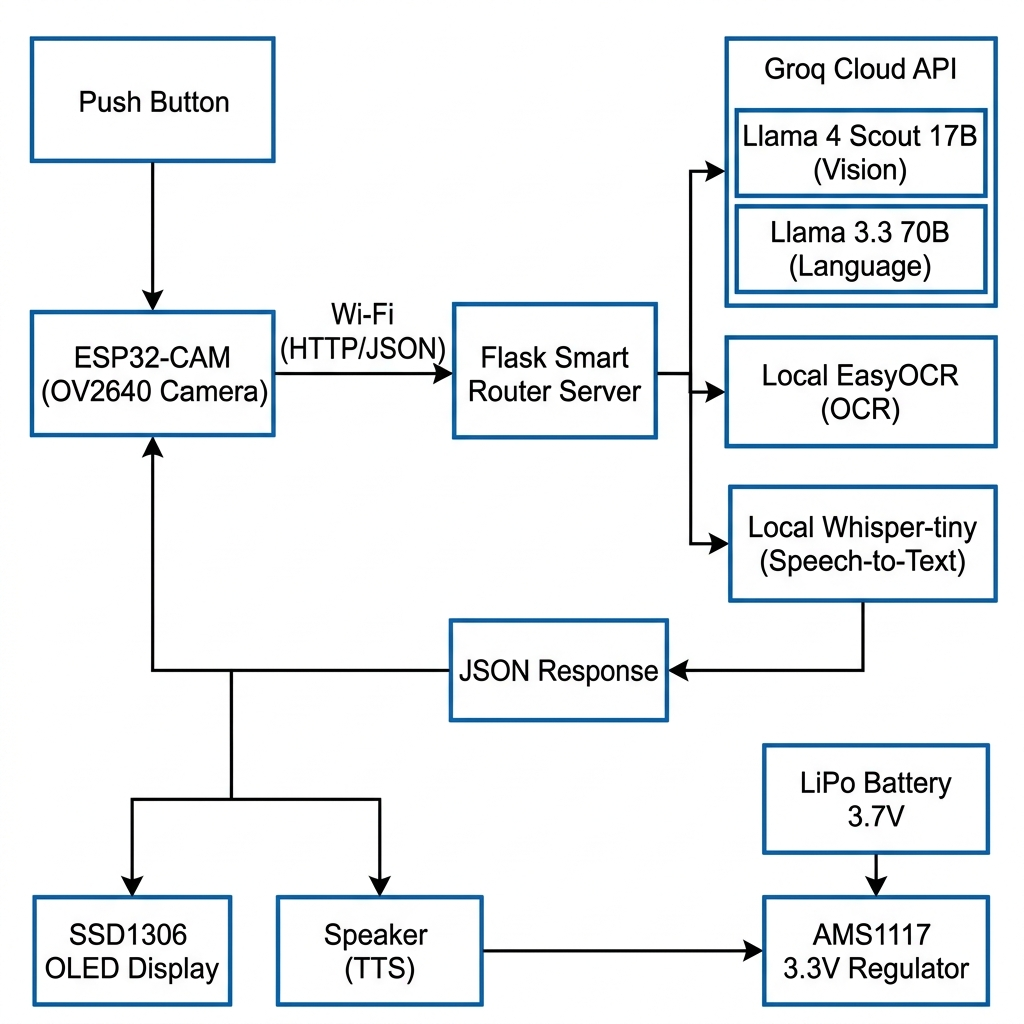
\includegraphics[width=0.85\textwidth]{images/block_diagram.png}
\caption{System Architecture Block Diagram --- AI-Powered Smart Glasses Using ESP32-CAM}
\end{figure}

The block diagram illustrates the complete data flow from user input through AI processing to output delivery. The system is organized into two major domains: the \textit{Wearable Device Domain} (ESP32-CAM with peripherals) and the \textit{Backend Processing Domain} (Flask server with AI models). These domains communicate wirelessly via Wi-Fi using HTTP/REST protocol.

In the Wearable Device Domain, the ESP32-CAM serves as the central hub connecting all hardware peripherals---the OV2640 camera (via 8-bit parallel bus), the INMP441 microphone (via I2S), the SSD1306 OLED display (via I2C), the micro speaker (via DAC/PWM), and the push buttons (via GPIO). The power supply subsystem (LiPo battery, TP4056 charger, AMS1117 regulator) provides regulated 3.3V power to all components.

In the Backend Processing Domain, the Flask Smart Router receives HTTP requests from the ESP32 and dispatches them to the appropriate AI model. Cloud-based models (Llama 4 Scout 17B, Llama 3.3 70B) are accessed via the Groq API over HTTPS, while local models (EasyOCR, Whisper-tiny) run on the backend server's GPU. The Smart Router manages the lifecycle of local models, ensuring memory-efficient operation.

\section{Power Supply Subsystem}
The power supply subsystem will provide stable, regulated power to all electronic components of the smart glasses. It consists of three key components:

\begin{itemize}[leftmargin=1.5cm]
\item \textbf{LiPo Battery (3.7V, 1000 mAh):} The primary energy storage element. Lithium polymer chemistry provides high energy density in a compact, lightweight form factor suitable for wearable applications. The battery will provide a nominal voltage of 3.7V, ranging from 4.2V (fully charged) to 3.0V (minimum safe discharge level).

\item \textbf{TP4056 Charging Module:} Will provide safe, controlled charging of the LiPo battery via USB micro connector. The module implements constant-current/constant-voltage (CC/CV) charging with automatic cutoff at 4.2V to prevent overcharging. Built-in undervoltage protection will disconnect the load at 2.5V to prevent deep discharge damage. A dual-LED indicator (red for charging, blue/green for fully charged) will provide charging status feedback.

\item \textbf{AMS1117-3.3V Voltage Regulator:} Will convert the variable battery voltage (3.0V--4.2V) to a stable 3.3V output required by the ESP32 and all peripheral components. The AMS1117 is a low-dropout (LDO) regulator with 1.1V dropout voltage and 800 mA maximum output current, providing adequate headroom for the system's peak current draw of approximately 346 mA. Two 100nF ceramic decoupling capacitors will be placed near the regulator output and the ESP32 power input pins to suppress high-frequency noise and prevent brownout resets during Wi-Fi transmission bursts, which can cause momentary current spikes of up to 500 mA.
\end{itemize}

\section{ESP32 Control Unit}
The ESP32-CAM module will serve as the central control unit, executing the firmware that orchestrates all hardware interactions and network communications. The dual-core Xtensa LX6 processor will allocate tasks across its two cores for optimal performance:

\begin{itemize}[leftmargin=1.5cm]
\item \textbf{Core 0:} Will handle the Wi-Fi protocol stack, TCP/IP networking, and HTTP client operations. This dedicated allocation ensures that network operations do not interrupt time-sensitive peripheral communication.

\item \textbf{Core 1:} Will run the main application loop, including camera frame capture, I2C display rendering, I2S microphone sampling, GPIO button interrupt handling, JSON parsing, and application state management.
\end{itemize}

The firmware will manage the following operations:

\begin{itemize}[leftmargin=1.5cm]
\item Camera frame buffer allocation and JPEG compression using the ESP32's hardware JPEG encoder
\item I2C bus initialization for the OLED display (SDA: GPIO 14, SCL: GPIO 15) at 400 kHz
\item I2S peripheral configuration for the INMP441 microphone (WS: GPIO 25, SCK: GPIO 26, SD: GPIO 22) at 16 kHz sample rate
\item GPIO interrupt handlers for push button presses (Button 1: GPIO 12, Button 2: GPIO 13) with 200 ms software debouncing
\item HTTP POST client operations for server communication using the ESP32 HTTPClient library
\item JSON response parsing using the ArduinoJson library (v6.x) for extracting AI response text
\item OLED display rendering with automatic word wrapping, scrolling, and mode status indicators
\end{itemize}

\section{Sensor Subsystem}
The system will employ two primary sensing modalities to capture visual and auditory input from the user's environment:

\begin{itemize}[leftmargin=1.5cm]
\item \textbf{Visual Sensor (OV2640 Camera):} Will capture images in JPEG format at 640$\times$480 resolution using the ESP32-CAM's integrated camera module. The camera interfaces with the ESP32 through an 8-bit parallel data bus with four timing signals: XCLK (20 MHz external clock generated by the ESP32), PCLK (pixel clock output from the camera), VSYNC (vertical sync indicating frame boundaries), and HREF (horizontal reference indicating valid pixel data). The camera's built-in auto-exposure (AEC), auto-gain (AGC), and auto-white-balance (AWB) algorithms will ensure consistent image quality across varying lighting conditions---from bright outdoor sunlight to dim indoor environments. The JPEG compression hardware within the OV2640 will reduce raw image data from approximately 600 KB (640$\times$480$\times$2 bytes in RGB565) to approximately 30--50 KB, enabling efficient wireless transmission.

\item \textbf{Audio Sensor (INMP441 Microphone):} Will capture audio data through the I2S digital interface at 16 kHz sample rate with 24-bit resolution per sample. The I2S bus uses three signal lines: WS (Word Select/LRCLK on GPIO 25) to indicate left/right channel selection, SCK (Serial Clock/BCLK on GPIO 26) for bit-level synchronization, and SD (Serial Data on GPIO 22) for the actual audio data stream. The digital MEMS microphone provides 61 dB signal-to-noise ratio, ensuring clear voice capture even in moderately noisy environments. The omnidirectional pickup pattern will capture the user's voice from any direction, accommodating natural speaking positions.
\end{itemize}

\section{OLED Display Subsystem}
The SSD1306 OLED display will be driven via the I2C protocol at device address 0x3C with 400 kHz clock speed, using the Adafruit SSD1306 library for graphics rendering. The display will support three rendering modes:

\begin{itemize}[leftmargin=1.5cm]
\item \textbf{Text Mode:} Will render AI response text using a 6$\times$8 pixel monospace font, providing approximately 21 characters per line and 8 lines per screen. Automatic word wrapping at word boundaries will ensure readable text presentation. Responses exceeding the 8-line capacity will be displayed with automatic vertical scrolling at a configurable speed.

\item \textbf{Status Mode:} Will display the current operating mode (Scene, OCR, Voice, Q\&A, Translate) as a header bar with the battery voltage indicator on the right side. This mode will be active between AI requests, providing the user with feedback about the current system state.

\item \textbf{Processing Mode:} Will display an animated loading indicator while the system is waiting for the AI response from the backend server. This will provide visual feedback that the system is actively processing the request and prevent the user from triggering duplicate requests.
\end{itemize}

The self-emitting OLED technology provides high contrast (10,000:1 ratio) and wide viewing angles (up to 160 degrees), ensuring visibility in both bright outdoor and dim indoor environments. The display draws only 20 mA at full brightness, contributing minimally to overall power consumption.

\section{Flask Web Server (Smart Router)}
The Flask web server will serve as the intelligence hub of the system. It will expose six API endpoints (five functional endpoints plus one health check) and implement the Smart Routing logic that is the core architectural innovation of this project.

\subsection*{Server Architecture Layers:}
The backend server will be organized into four distinct architectural layers, each with clearly defined responsibilities:

\begin{enumerate}[leftmargin=1.5cm]
\item \textbf{Request Handler Layer:} Will receive incoming HTTP POST requests, validate the Content-Type header (application/json), parse the JSON payload, validate the presence of required fields (image data, request type), and extract the Base64-encoded payload for processing. Malformed requests will receive HTTP 400 (Bad Request) responses with descriptive error messages. Requests to undefined endpoints will receive HTTP 404 (Not Found) responses.

\item \textbf{Smart Router Layer:} Will determine the appropriate AI model based on the endpoint called, manage the model loading and unloading lifecycle, and track system resource usage via the psutil library and PyTorch's CUDA memory tracking utilities (\texttt{torch.cuda.memory\_allocated()}, \texttt{torch.cuda.memory\_reserved()}). The router will maintain an internal model registry that tracks which local model (if any) is currently loaded in GPU memory. Before loading a new local model, the router will ensure any previously loaded model is fully unloaded and its memory is freed.

\item \textbf{AI Model Layer:} Will contain wrapper functions for each AI model, providing a unified interface for the Smart Router:
\begin{itemize}
\item Groq API client wrapper for cloud models (Llama 4 Scout 17B for vision, Llama 3.3 70B for language tasks)
\item EasyOCR reader instance wrapper for optical character recognition (supports English and Hindi)
\item Whisper model instance wrapper for speech-to-text transcription
\end{itemize}
Each wrapper function will accept raw input data (decoded image bytes or audio samples) and return a standardized response dictionary containing the AI-generated text and processing metadata.

\item \textbf{Response Layer:} Will format AI model outputs into standardized JSON responses containing four fields: \texttt{status} (success/error string), \texttt{response} (AI-generated text), \texttt{processing\_time\_ms} (elapsed time in milliseconds), and \texttt{memory\_usage\_mb} (current GPU memory allocation in megabytes). This standardized format will enable the ESP32 firmware to parse responses from any endpoint using a single JSON parsing routine.
\end{enumerate}
